% Copyright 2004 by Till Tantau <tantau@users.sourceforge.net>.
%
% In principle, this file can be redistributed and/or modified under
% the terms of the GNU Public License, version 2.
%
% However, this file is supposed to be a template to be modified
% for your own needs. For this reason, if you use this file as a
% template and not specifically distribute it as part of a another
% package/program, I grant the extra permission to freely copy and
% modify this file as you see fit and even to delete this copyright
% notice. 

\documentclass{beamer}

% There are many different themes available for Beamer. A comprehensive
% list with examples is given here:
% http://deic.uab.es/~iblanes/beamer_gallery/index_by_theme.html
% You can uncomment the themes below if you would like to use a different
% one:
%\usetheme{AnnArbor}
%\usetheme{Antibes}
%\usetheme{Bergen}
%\usetheme{Berkeley}
%\usetheme{Berlin}
%\usetheme{Boadilla}
%\usetheme{boxes}
%\usetheme{CambridgeUS}
%\usetheme{Copenhagen}
%\usetheme{Darmstadt}
%\usetheme{default}
%\usetheme{Frankfurt}
%\usetheme{Goettingen}
%\usetheme{Hannover}
%\usetheme{Ilmenau}
%\usetheme{JuanLesPins}
%\usetheme{Luebeck}
\usetheme{Madrid}
%\usetheme{Malmoe}
%\usetheme{Marburg}
%\usetheme{Montpellier}
%\usetheme{PaloAlto}
%\usetheme{Pittsburgh}
%\usetheme{Rochester}
%\usetheme{Singapore}
%\usetheme{Szeged}
%\usetheme{Warsaw}

\usepackage{kotex}
\usepackage{braket}
\usepackage{array}
\usepackage{calc}
\usepackage{datetime}
\usepackage{dsfont}
\usepackage{amsmath}
\usepackage{listings}


\title{Lecture 3 : 행렬/선형대수학의 응용}

% A subtitle is optional and this may be deleted
\subtitle{Fastcampus Math Camp}

\author{신승우}
% - Give the names in the same order as the appear in the paper.
% - Use the \inst{?} command only if the authors have different
%   affiliation.

% \institute[Universities of Somewhere and Elsewhere] % (optional, but mostly needed)
% {
  % \inst{1}%
  % Department of Computer Science\\
  % University of Somewhere
  % \and
  % \inst{2}%
  % Department of Theoretical Philosophy\\
  % University of Elsewhere}
% - Use the \inst command only if there are several affiliations.
% - Keep it simple, no one is interested in your street address.

% - Either use conference name or its abbreviation.
% - Not really informative to the audience, more for people (including
%   yourself) who are reading the slides online

\subject{Theoretical Computer Science}

% This is only inserted into the PDF information catalog. Can be left
% out. 

% If you have a file called "university-logo-filename.xxx", where xxx
% is a graphic format that can be processed by latex or pdflatex,
% resp., then you can add a logo as follows:

% \pgfdeclareimage[height=0.5cm]{university-logo}{university-logo-filename}
% \logo{\pgfuseimage{university-logo}}

% Delete this, if you do not want the table of contents to pop up at
% the beginning of each subsection:


\AtBeginSection[]
{
  \begin{frame}<beamer>{Outline}
    \tableofcontents[currentsection,hideallsubsections]
  \end{frame}
}

% Let's get started
\begin{document}

\begin{frame}
  \titlepage
\end{frame}

\begin{frame}{Outline}
  \tableofcontents[hideallsubsections]
  % You might wish to add the option [pausesections]
\end{frame}

% Section and subsections will appear in the presentation overview
% and table of contents.

\begin{frame}
지난시간에는 

\begin{itemize}
\item 수식의 파싱 
\item 벡터
\begin{itemize} 
\item 벡터의 정의와 연산 
\item 벡터의 선형독립 및 span 
\item 좌표계 및 기저 
\item 몇 가지 예시 
\end{itemize}
\end{itemize}

이번시간에는 

\begin{itemize} 
\item 행렬
\begin{itemize} 
\item 행렬의 정의와 연산 
\item 행렬과 선형변환 
\end{itemize} 
\item 추상 벡터 공간 
\end{itemize}

\end{frame}

\section{행렬} 



\subsection{행렬의 정의} 
\begin{frame}{행렬의 정의}
\begin{block}{행렬}  
행렬은 벡터의 모임 $M = [\vec{v_i}]$로 정의한다. 이 때, 각 $\vec{v_i}$를 column 벡터라고 한다. $M_{ij} = v_j$의 i번째 원소로 생각한다. 벡터가 n-벡터이고, m개의 column 벡터로 이루어져 있는 행렬을 $m \times n$ 행렬이라고 한다. 
\end{block}
이와 비슷하게, row 벡터로 정의할 수도 있다. 
\end{frame}

\subsection{행렬의 연산}

\begin{frame}{행렬의 연산 : 덧셈/뺄셈/스칼라배} 
\begin{itemize} 
\item 덧셈/뺄셈 
\item 스칼라배
\end{itemize}
\end{frame}

\begin{frame}{행렬의 연산 : 곱셈} 
\begin{itemize} 
\item 행렬-행렬 곱셉 : $C = A\times B$ 라 하자. 이 때, A가 $m \times n$ 행렬이고 B가 $p \times k$ 행렬일 때, $n=p$ 여야 곱셉이 가능하며, 결과는 $m \times k$ 행렬이 된다. $C_{ij} = \sum^m A_{ik} B_{kj}$ 로 정의된다. 행렬의 곱셈은 일반적으로 교환법칙이 성립하지 않으나, 1) 결합법칙은 성립한다. 
\item 행렬-벡터 곱셈 : 행렬-행렬 곱셈의 특이한 케이스이다. 
\end{itemize}

위 행렬의 곱셈의 정의에서, $I_{ij} = \delta_{ij}$인 행렬은 임의의 행렬 A에 대해서 2) $AI = IA = A$이다. 이 I를 단위행렬이라고 한다. 
\end{frame}

\begin{frame}{Einstein Notation의 소개} 

앞으로 다룰 대부분의 합은 대개의 경우 벡터나 행렬의 원소들의 곱으로 나타내어진다. 따라서, 공통된 첨자가 있을 경우 합 표기를 따로 명시하지 않는 한 생략한다. 예를 들어서, 두 벡터 $\vec{v} = (v_1, v_2, ..., v_n), \vec{u} = (u_1, u_2, ..., u_n)$의 내적의 경우 원래대로 표기하면 

\begin{equation} 
\vec{v} \bullet \vec{u} = \sum^{n}_{i=1} v_i u_i 
\end{equation}

이나, 이제부터는 

\begin{equation} 
\vec{v} \bullet \vec{u} =  v_i u_i 
\end{equation}

로 표기할 것이다.

\end{frame}

\begin{frame}{Proof of 1)} 

m by n 행렬 A, n by p 행렬 B, p by q 행렬 C에 대해서 

\begin{eqnarray} 
[(AB)C]_{ij} & = & (AB)_{ik} c_{kj} \\
& = & a_{il}b_{lk}c_{kj}  \\
& = & a_{ik} (BC)_{kj}  = [A(BC)]_{ij}
\end{eqnarray}
이다. 따라서 결합법칙이 성립한다. 
\end{frame}


\begin{frame}{Proof of 2)} 

n by n 행렬 A와 I에 대해서, 

\begin{eqnarray} 
(AI)_{ij} & = & a_{ik} I_{kj} \\
& = & a_{ik}\delta_{kj}  \\
& = & a_{ij} = A_{ij} 
\end{eqnarray}

이며, 비슷하게 

\begin{eqnarray} 
(IA)_{ij} & = & \delta_{ik}a_{kj} \\ 
& = & a_{ik}\delta_{kj}  \\
& = & a_{ij} = A_{ij}
\end{eqnarray}
\end{frame}


\begin{frame}{행렬의 곱셈}

\begin{itemize}
\item Naive Approach : $O(n^3)$
\item Strassen's Algorithm : $O(n^{2.8})$
\end{itemize}
\end{frame}

\begin{frame}{행렬의 곱셈 : Strassen's Algorithm} 

\begin{centering}
A = 
$ \left[ \begin{matrix}
A_{11} & A_{12}  \\
A_{21} & A_{22} 
\end{matrix} \right] $ \\

B = 
$ \left[ \begin{matrix}
B_{11} & B_{12}  \\
B_{21} & B_{22} 
\end{matrix} \right] $ \\

C = AB =  
$ \left[ \begin{matrix}
C_{11} & C_{12}  \\
C_{21} & C_{22} 
\end{matrix} \right] $ \\
\end{centering}

\end{frame}

\begin{frame}{행렬의 곱셈 : Strassen's Algorithm} 
1) 이 때, naive한 C의 계산은 다음과 같다. 
\begin{eqnarray} 
C_{11} & = & A_{11}B_{11} + A_{12}B_{21} \\
C_{12} & = & A_{11}B_{12} + A_{12}B_{22} \\
C_{21} & = & A_{21}B_{11} + A_{22}B_{21} \\
C_{22} & = & A_{21}B_{12} + A_{22}B_{22} 
\end{eqnarray}

이 경우, C를 계산하기 위해서는 8번의 곱하기와 4번의 더하기가 필요하다. 이 때, 곱하기가 비싼 계산이므로, 곱하기의 수를 줄이는 방법에 대해서 생각해 보자. 

\end{frame}

% \begin{frame}{Proof of 1)} 
% 행렬의 크기가 $2^n$ by $2^n$일 때, 수학적 귀납법을 이용하여 증명한다. 여기서는 제 2 수하적 귀납법을 이용하고자 한다. \footnote{수학적 귀납법은 제 1, 제 2 다 어떤 명제 f(n)이 n이 1일때 성립함을 보인다. 그 후, 제 1 수학적 귀납법은 f(n-1)일때 성립하면 f(n)임을 보인다. 제 2 수학적 귀납법은 n-1 이하의 모든 수 i에 대해서 f(i)가 성립함을 보이는 것이다.} 

% 행렬의 크기가 2 by 2일때는 행렬의 곱셈과 같으므로 자명하게 성립한다. 
% 행렬의 크기가 $2^{n-1}$ by $2^{n-1}$일 때 성립한다고 가정하자. 이 때 
% \end{frame}

\begin{frame}{행렬의 곱셈 : Strassen's Algorithm} 

\begin{eqnarray} 
M_1 & = & (A_{11} + A_{22}) (B_{11} + B_{22}) \\
M_2 & = & (A_{21} + A_{22}) B_{11} \\
M_3 & = & A_{11} (B_{12} - B_{22}) \\
M_4 & = & A_{22} (B_{21} - B_{11}) \\
M_5 & = & (A_{11} + A_{12}) B_{22} \\
M_6 & = & (A_{21} - A_{11}) (B_{11} + B_{12}) \\
M_7 & = & (A_{12} - A_{22}) (B_{21} + B_{22}) 
\end{eqnarray}


으로 보조 행렬들을 만들 때, 다음이 성립한다. 
\end{frame}



\begin{frame}{행렬의 곱셈 : Strassen's Algorithm} 

\begin{eqnarray} 
C_{11} & = & M_1 + M_4 - M_5 + M_7 \\
C_{12} & = & M_3 + M_5 \\
C_{21} & = & M_2 + M_4 \\
C_{22} & = & M_1 - M_2 + M_3 + M_6
\end{eqnarray}

이를 이용해서, 곱셈을 덜 하고 덧셈을 더 해서 행렬의 곱셈을 최적화할 수 있다. 정확하게는 7번의 곱셈과 18번의 덧셈이 필요하다. 만약 행렬의 크기가 짝수가 아니라면, 필요한 만큼 0을 덧붙여 계산한다. 

\end{frame}

\begin{frame}{Complexity of Strassen's Algorithm} 

$T(n) = 7*T(n/2) + 18n^2$ 으로 계산된다. 이는 $n=2^k$로 치환하고 계산하면 $O(n^{log_2 7})$을 얻을 수 있다. 

\end{frame} 


% \begin{frame}{Dive more : Application of Parallel Computing}


% \end{frame}


\begin{frame}{행렬의 연산 : elementary operations} 
행렬의 elementary operation에는 다음의 3가지가 있다. 

\begin{itemize} 
\item 행/열 바꾸기 
\item 행/열 더하기
\item 특정 행/열에 상수 곱하기
\end{itemize}

위 연산들을 종합하면, 행렬의 row vector들의 선형결합으로 특정 row vector을 대체하는 것을 말한다. 이는 원 행렬에 적절한 행렬을 곱하여 얻을 수 있다. 

\end{frame}

\begin{frame}{행렬의 연산 : elementary operation } 

row vector $\vec{v}_i$로 이루어진 행렬 A가 있다고 하자. 이 때, row vector $\vec{u}_j = c_{ji} \vec{v}_i$를 row vector로 가지는 행렬 B는 

B = CA 

를 만족한다. 이 때 1) $C_{ij} = c_{ij}$이며, C는 정사각행렬이다.

\end{frame}

\begin{frame}{ Proof of 1)} 
곱셈의 정의를 그대로 쓰면, 
$(CA)_{i} =  c_{ik} a_{k} $
이므로 성립한다. 
\end{frame}

\begin{frame}{행렬의 연산 : elementary operation의 예시} 


\begin{itemize} 
\item 행/열 바꾸기 


$ \left[ \begin{matrix}
0 & 1  \\
1 & 0 
\end{matrix} \right] \times
\left[ \begin{matrix}
2 & 1 & 3   \\
-1 & 3 & 2 
\end{matrix} \right] = 
\left[ \begin{matrix}
-1 & 3 & 2   \\
2 & 1 & 3 
\end{matrix} \right] $

\item 행/열 더하기

$ \left[ \begin{matrix}
1 & 1  \\
0 & 1 
\end{matrix} \right] \times
\left[ \begin{matrix}
2 & 1 & 3   \\
-1 & 3 & 2 
\end{matrix} \right] = 
\left[ \begin{matrix}
1 & 4 & 5   \\
-1 & 3 & 2 
\end{matrix} \right] $

\item 상수 곱하기

$ \left[ \begin{matrix}
1 & 0  \\
0 & 3 
\end{matrix} \right] \times
\left[ \begin{matrix}
2 & 1 & 3   \\
-1 & 3 & 2 
\end{matrix} \right] = 
\left[ \begin{matrix}
2 & 1 & 3   \\
-3 & 9 & 6 
\end{matrix} \right] $

\item 선형결합 $\vec{u}_1 = \vec{v}_1, \vec{u}_2 = \vec{v}_1 + 3\vec{v}_2$ 의 경우,

$ 
\left[ \begin{matrix}
1 & 0  \\
1 & 1 
\end{matrix} \right] \times 
\left[ \begin{matrix}
1 & 0  \\
0 & 3 
\end{matrix} \right] \times
\left[ \begin{matrix}
2 & 1 & 3   \\
-1 & 3 & 2 
\end{matrix} \right] = 
\left[ \begin{matrix}
2 & 1 & 3   \\
-1 & 10 & 9 
\end{matrix} \right] $

\end{itemize}
\end{frame}

\begin{frame}{행렬의 연산 : 가우스 소거법(실습)} 
가우스 소거법은 elementary operation의 연장선상으로, 행렬을 reduced row echelon 행렬로 만드는 것을 말한다. reduced row echelon 행렬을 정의하기 위해서 우선 행렬의 i번째 행의 선행 계수를 다음과 같이 정의하자. 

$j(i) = min(j \leq n, M_{ij} \neq 0)$

이 때, 다음 조건을 만족시키는 행렬을 row echelon 행렬이라고 하며, 각 행의 선행 계수에 해당하는 원소가 1이며 그 열에서는 1 하나를 빼고 모든 원소가 0인 경우 reduced row echelon 행렬이라고 한다. 

\begin{itemize} 
\item 행의 모든 원소가 0이면, 그 행보다 아래에 있는 행의 모든 원소 또한 0이다. 
\item $i<k, j(i) < j(k)$ 이다. 
\end{itemize}

즉, 0이 아닌 숫자가 사다리꼴로 배열되어 있는 행렬을 말한다. 
\end{frame}

\begin{frame}{행렬의 연산 : 가우스 소거법(실습)} 

가우스 소거법은 다음과 같다. 

\begin{itemize} 
\item j번째 행에 대해서, 첫번째 행부터 순차적으로 
\begin{itemize} 
\item 선행 계수가 존재하는 가장 작은 열수를 찾는다. 
\item 현재 행과 찾아진 행을 치환한다. 
\item 선행계수에 해당하는 열에서 현재 행보다 아래 행들의 해당 열을 0으로 만든다. 
\end{itemize}
\end{itemize}

\end{frame}

\begin{frame}[allowframebreaks]{가우스 소거법 실습} 

지금부터 30분 동안 진행합니다. 짜는 과정에서 다음의 보조함수들을 짜는 것을 추천합니다. 

\begin{itemize} 
\item 선행 계수가 존재하는 가장 작은 열을 찾는 함수(\_find\_leading\_row)
\item elementary operation들과 그에 해당하는 행렬 
\begin{itemize} 
\item 행 바꾸기 (change\_row)
\item 행에 상수 곱하기 (multiply\_row)
\item 행에 다른 행 더하기 (add\_row)
\end{itemize}
\item Identity 행렬 출력하는 static method(PyMatrix.identity)
\end{itemize}

출력은 리스트와 PyMatrix 인스턴스 하나로, 다음과 같습니다. 

\begin{itemize} 
\item 리스트 : 어떤 elementary operation을 했는지 대응되는 행렬의 리스트
\item 가우스 소거의 결과 행렬 
\end{itemize}

다 한 후, 시간이 남으면 나온 결과물을 검증하는 코드도 짜서 검증해보시면 좋습니다. 

\end{frame}




\begin{frame}{행렬의 연산 : trace, transpose} 
\begin{itemize} 
\item trace : $tr(A) = \sum_i A_{ii}$
\item transpose : $(A^{T})_{ij} = A_{ji}$
\end{itemize}

임의의 행렬 A,B에 대해서 
\begin{itemize}
\item $(AB)^T = B^TA^T$
\item $tr(AB) = tr(BA)$
\end{itemize}  
\end{frame}

\begin{frame}{Proof of 1)} 
\begin{eqnarray}
((AB)^T)_{ij} &=& (AB)_{ji} \\
&=& a_{jk}b_{ki} \\
&=& a^T_{kj}b^T_{ik} \\
&=& b^T_{ik} a^T_{kj} \\
&=& (B^T A^T)_{ij}
\end{eqnarray}

이므로 성립한다. 
\end{frame}


\begin{frame}{Proof of 2)} 
\begin{eqnarray}
tr(AB) &=& \sum AB_{ii} \\
&=& a_{ik}b_{ki} \\
&=& b_{ki}a_{ik} \\
&=& \sum BA_{kk} = tr(BA)
\end{eqnarray}
\end{frame}



\begin{frame}{행렬의 연산 : determinant} 
행렬식은 재귀적으로 정의되며, 정사각행렬에서만 정의된다. 행렬 A의 행렬식 $det(A)$는 
\begin{itemize} 
\item 행렬의 size가 (1,1) : $A_{11}$
\item 행렬의 size가 (n,n) : $\sum^{n}_{i=1}(-1)^n det(minor(A, 1, i))$
여기서, $minor(A, i, j)$는 i번째 row와 j번째 column을 제거한 행렬을 말한다. 
\end{itemize}

1) 두 행렬 A,B에 대해서 $det(AB) = det(A) det(B)$ 이다. 
\end{frame}


\begin{frame}{행렬의 연산 : 역행렬} 

행렬 A의 역행렬은 $A^{-1}$ 이라고 표기하며, $AA^{-1} = A^{-1}A = I$ 를 만족한다. A가 역행렬을 가지면, A는 invertible matrix라고 한다. 

역행렬은 다음의 성질들을 가진다. 

\begin{itemize} 
\item $A^{-1}$이 존재하려면 A는 정사각행렬이여야 한다. 
\item $(A^{-1})^{-1} = A$
\item A의 역행렬은 유일하다. 
\item A의 역행렬이 있다면 $(A^T)^{-1} = (A^{-1})^T$
\item 역행렬이 있는 행렬은 행렬식이 0이 아니며, 역도 성립한다. 
\end{itemize} 

\end{frame}

\begin{frame}{Proof of 3)}
서로 다른 두 행렬 B,C가 A의 역행렬이라고 하면, 

B = BI = B(AC) = (BA)C = C 

이므로 B=C이다. 따라서 모순이므로 역행렬은 유일하다. 
\end{frame}

\begin{frame}{Proof of 4)} 
행렬 A에 대해서, 

$(A A^{-1})^T = (A^{-1})^T A^T  = I^T = I$ 이므로 성립한다. 
\end{frame}


\begin{frame}{역행렬을 찾는 법}
행렬 A에 대해서 역행렬을 찾는 법을 생각해보자. 먼저, A가 $\vec{v}_i$의 row vector로 이루어져 있다고 생각하자. 이 때, 어떤 elementary operation들을 수행하여 A를 I로 만들 수 있다면, 그 elemantary operation들에 해당하는 행렬이 역행렬이 될 것이다.  

예를 들어서, 

$
\left[ \begin{matrix}
1 & 1  \\
0 & 1 
\end{matrix} \right] \times
\left[ \begin{matrix}
1 & -1  \\
0 & 1 
\end{matrix} \right] =
\left[ \begin{matrix}
1 & 0  \\
0 & 1 
\end{matrix} \right] $ 

이므로 



$\left[ \begin{matrix}
1 & 1  \\
0 & 1 
\end{matrix} \right] ^{-1} = 
\left[ \begin{matrix}
1 & -1  \\
0 & 1 
\end{matrix} \right] $

이다. 즉, 역행렬을 찾는 것은 elementary operation들을 수행해서 행렬을 I로 만드는 것과 같다. 이제 본격적으로 어떻게 역행렬을 찾는지 알아보자. 

\end{frame}

\begin{frame}{역행렬 찾기} 
행렬 A에 대해서 다음의 과정을 시행한다. 
\begin{itemize} 
\item for i = 1, 2, ... , n, 
\begin{itemize}
\item $a_{ii} = 1$이 되게 한다. 이 때, 
\begin{itemize} 
\item 1) 만약 $a_{ji}$이 모두 0이라면, elementary operation을 이용하여 $a_{ii} = 1$이 되게 하는 것은 불가능하다. 따라서 역행렬도 존재하지 않는다. 
\item 하나라도 0이 아니라면, 그 행을 이용하여 $a_{ii} = 1$로 만든다. 
\end{itemize}
\item 그 후 i가 아닌 모든 j에 대해서, $a_{ji}$가 0이 되도록 만든다. 
\end{itemize}
\end{itemize}

\end{frame}



% \subsection{Row/Column Space}

% \begin{frame}{Row Space}

% \begin{itemize}
% \item 
% \end{itemize}

% \end{frame} 

% \begin{frame}{Column Space} 

% \end{frame}

% \begin{frame}{Rank-Nullity Theorem} 

% \end{frame}

% \begin{frame}{Inverse Matrix Revisited} 

% \end{frame}



\subsection{선형변환과의 관계} 

\begin{frame}{선형변환} 

$V=\mathds{R}^n$에서 $W=\mathds{R}^m$으로의 선형변환은 V의 원소를 벡터공간 W의 원소로 대응시키는 함수 중 다음을 만족하는 함수를 말한다. 
\begin{itemize} 
\item $f(\vec{u} + \vec{v}) = f(\vec{u}) + f(\vec{v})$
\item $f(c\vec{u}) = c f(\vec{u}) $
\end{itemize}
\end{frame}

\begin{frame}{선형변환과 행렬} 
선형변환은 행렬로 볼 수 있다. 더 정확하게는, 1) $V=\mathds{R}^n$에서 $W=\mathds{R}^m$으로의 선형변환은 m by n 행렬로 볼 수 있다. 
\end{frame}

\begin{frame}[allowframebreaks]{Construction from Linear Transformation to Matrix  }

V의 기저 $\{\vec{v}_i\}$를 생각하자. 이 때, V의 임의의 원소인 $\vec{v}$는 다음과 같이 쓸 수 있다. 

\begin{equation} 
\vec{v} = c_i \vec{v}_i
\end{equation}

이 때, 선형변환 $f:V \rightarrow W$에 대해서 $f(\vec{v})$는 

\begin{equation}
f(\vec{v}) = f(c_i \vec{v}_i) = c_i f(\vec{v}_i)
\end{equation} 

로 생각할 수 있다. 이제, W의 기저 $\{\vec{w}_i\}$를 생각하자. $f(\vec{v}_i)$는 W의 원소이므로 다음과 같이 쓸 수 있다. 

\begin{equation}
f(\vec{v}_i) = d_ij \vec{w}_j
\end{equation} 

이에 착안해서, $d_{ij}$를 이용해서 행렬 D를 만들면, n by m 행렬이 된다. 이 행렬을 Transformation Matrix라고 한다. 이 행렬을 이용하면, $\vec{v} \in V$에 대해서 $f(\vec{v}) =  D \vec{v}$ 임을 알 수 있다. 

\end{frame}

\begin{frame}{선형변환의 예시 : 2차원 회전변환} 
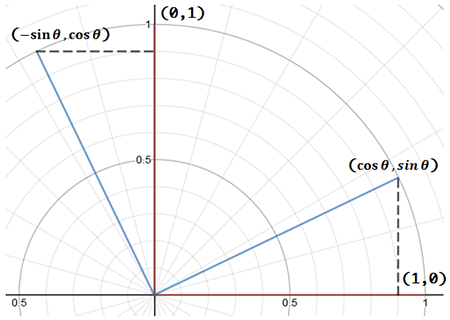
\includegraphics[width=10cm,keepaspectratio]{rot}

\end{frame}

\begin{frame}{선형변환의 예시 : 2차원 회전변환}

$T_{\theta} = 
\left[ \begin{matrix}
cos \theta & - sin \theta  \\
sin \theta & cos \theta 
\end{matrix} \right] $
\end{frame}

\begin{frame}{행렬의 연산을 이용한 선형변환}
선형변환이라는 함수가 행렬으로 표현가능하므로, 행렬의 연산을 이용해서 선형변환을 원하는 대로 만들 수 있다. 여기서는 크게 두 가지를 살펴보고자 한다. 

\begin{itemize} 
\item 합성함수와 행렬의 곱 
\item 역함수와 역행렬
\end{itemize}

이 두 가지 예시를 회전변환을 이용해서 살펴보고자 한다. 

\end{frame}

\begin{frame}{행렬 곱과 함성함수 } 

두 회전변환 

$T_{\alpha} = 
\left[ \begin{matrix}
cos \alpha & - sin \alpha  \\
sin \alpha & cos \alpha 
\end{matrix} \right] $

$T_{\beta} = 
\left[ \begin{matrix}
cos \beta & - sin \beta  \\
sin \beta & cos \beta 
\end{matrix} \right] $

가 있을 때, 두 변환행렬의 곱은 


$T_{\alpha} T_{\beta}  = 
\left[ \begin{matrix}
cos \alpha & - sin \alpha  \\
sin \alpha & cos \alpha 
\end{matrix} \right] \times 
\left[ \begin{matrix}
cos \beta & - sin \beta  \\
sin \beta & cos \beta 
\end{matrix} \right] = 
\left[ \begin{matrix}
cos \alpha cos \beta - sin \alpha sin \beta  & - cos \alpha sin \beta - sin \alpha cos \beta  \\
cos \alpha sin \beta + sin \alpha cos \beta  & cos \alpha cos \beta - sin \alpha sin \beta
\end{matrix} \right] 
 $
 
인데, 이는 삼각함수의 합차공식을 이용하면 $T_{\alpha + \beta}$임을 알 수 있다. 

\end{frame}

\begin{frame}{역행렬과 역함수} 
$T_{\alpha}$의 역행렬은 다음과 같이 구할 수 있다. 

$T_{\alpha} T^{-1}  = 
\left[ \begin{matrix}
cos \alpha & - sin \alpha  \\
sin \alpha & cos \alpha 
\end{matrix} \right] \times 
\left[ \begin{matrix}
cos \alpha & sin \alpha \\
- sin \alpha & cos \alpha
\end{matrix} \right] = I_2
$
인데, 이에서 $T^{-1} = T_{-\alpha}$임을 알 수 있다. 

\end{frame}


\subsection{행렬의 고유벡터와 고유값}

%https://math.stackexchange.com/questions/23312/what-is-the-importance-of-eigenvalues-eigenvectors

\begin{frame}{Definition of Eigen*} 
행렬 A에 대해서, 다음을 만족하는 $\lambda$와 $\vec{x}$들을 각각 고유값(eigenvalue)과 고유벡터(eigenvector)라고 한다. 

$ A \vec{x} = \lambda \vec{x}$ 

위 식을 다시 쓰면 

$ (A-\lambda I) \vec{x} = 0 $ 

이며, 여기서 $det(A-\lambda I)=0$를 특성방정식이라 한다. 이 때 특성방정식의 해는 고유값이 되며, 이에 따라 고유벡터를 계산할 수 있다. 

고유벡터들로 span되는 공간을 eigenspace라 한다. 
\end{frame}

\begin{frame}[allowframebreaks]{Motivation of Eigen*}
위에서 다룬 회전변환 행렬 T를 생각해 보자. 


$T_{\theta} = 
\left[ \begin{matrix}
cos \theta & - sin \theta  \\
sin \theta & cos \theta 
\end{matrix} \right] $

이 때, 회전의 축을 어떻게 구할 수 있을까? 회전의 축은 회전 전후에도 변화가 없을 것이다. 따라서, 회전의 축을 벡터 $\vec{a}$라 하면, $T\vec{a} = \vec{a}$ 임이 성립해야 한다. 이 경우, 이를 만족하는 벡터 a는 0벡터 뿐이다. 그렇다면 이는 무슨 의미를 가질까? 이는 회전축이 z축이므로, 이를 나타내는 것으로 생각할 수 있다. 이는 다음의 3차원 회전변환 행렬을 생각해보면 조금 더 명확해진다. 

$T_{\theta} = 
\left[ \begin{matrix}
cos \theta & - sin \theta & 0 \\
sin \theta & cos \theta & 0 \\ 
0&0&1
\end{matrix} \right] $

이 경우 위와 같은 방정식을 풀면 z는 어떠한 수여도 가능하고, x와 y는 0임을 알 수 있다. 즉, z축이 회전의 축임을 알 수 있다. 

이는 일반적인 선형변환에서도 같다. 어떤 선형변환 R에 대해서, $R\vec{a} = \vec{a}$가 성립한다면, 그 벡터는 선형변환에 대해서 불변이다. 즉, 어떠한 행렬의 eigenvector는 그 행렬에 대응하는 선형변환의 축이라고 볼 수 있다. 


\end{frame}

\begin{frame}{직관적 이해 : Principal Component Analysis} 
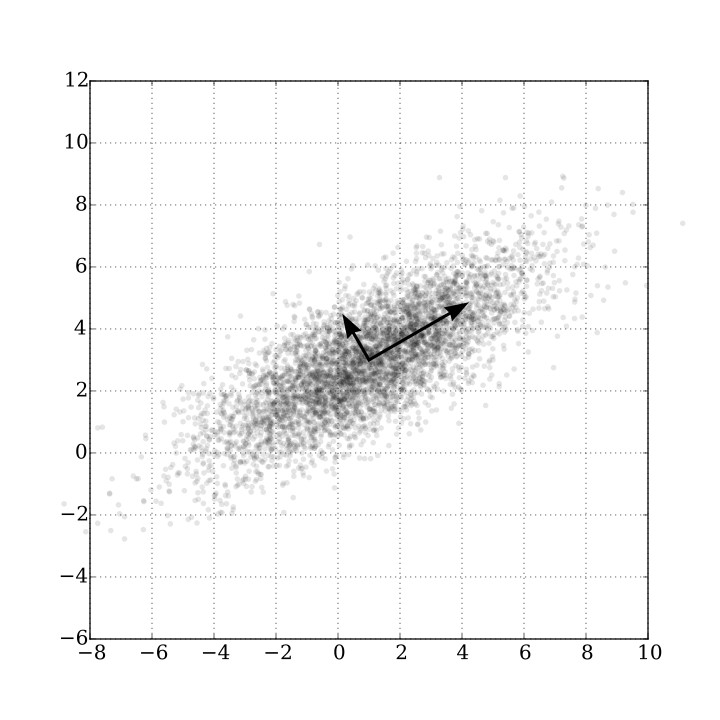
\includegraphics[height=8cm,keepaspectratio]{pca}
\end{frame}

\begin{frame}{Properties of Eigen*}
일반적으로, 다음 성질들이 성립한다. 

\begin{itemize} 
\item $A^T$의 고유값과 고유벡터는 A와 같다. 
\item $A^TA$의 고유벡터는 A와 같고, 고유값은 제곱값이다. 
\item det(A)는 모든 고유값의 곱이다. 
\end{itemize}

\end{frame}

\begin{frame}[allowframebreaks]{Proof of 3)} 
어떤 행렬 A의 고유벡터를 $\vec{v}_i$, 고유값을 $\lambda_i$라 하자. 그러면 다음이 성립한다. 

\begin{eqnarray}
A \left[ \begin{matrix} 
\vec{v}_1 & \vec{v}_2 & ... & \vec{v}_n
\end{matrix} \right] 
 &=& A \left[ \begin{matrix} 
A\vec{v}_1 & A\vec{v}_2 & ... & A\vec{v}_n
\end{matrix} \right]  \\
&=& A \left[ \begin{matrix} 
\lambda_1 \vec{v}_1 & \lambda_2 \vec{v}_2 & ... & \lambda_n \vec{v}_n
\end{matrix} \right] \\
&=& \left[ \begin{matrix} 
\lambda_1 \vec{v}_1 & \lambda_2 \vec{v}_2 & ... & \lambda_n \vec{v}_n
\end{matrix} \right] 
\left[ \begin{matrix} 
\lambda_1 & 0 & ... & 0 \\
0 & \lambda_2 & ... & 0 \\
0 & 0 & ... & \lambda_n 
\end{matrix} \right] 
\end{eqnarray}

이다. 이 때, det(AB) = det(A) det(B)임을 이용하면 

\begin{eqnarray} 
& det(A) det \left( \left[ \begin{matrix} 
\vec{v}_1 & \vec{v}_2 & ... & \vec{v}_n
\end{matrix} \right]  \right) \\
= & det\left(\left[ \begin{matrix} 
\lambda_1 \vec{v}_1 & \lambda_2 \vec{v}_2 & ... & \lambda_n \vec{v}_n
\end{matrix} \right] \right)
det \left(\left[ \begin{matrix} 
\lambda_1 & 0 & ... & 0 \\
0 & \lambda_2 & ... & 0 \\
0 & 0 & ... & \lambda_n 
\end{matrix} \right] \right)\\
\end{eqnarray}

이므로, det(A)는 모든 고유값의 곱이 된다. 
\end{frame}

\begin{frame}{Eigendecomposition} 

Eigendecomposition은 어떤 행렬의 eigenvector들이 서로 선형독립일 때 가능하다. 위 증명에서, 
\begin{equation}
A \left[ \begin{matrix} 
\vec{v}_1 & \vec{v}_2 & ... & \vec{v}_n
\end{matrix} \right] 
= \left[ \begin{matrix} 
\lambda_1 \vec{v}_1 & \lambda_2 \vec{v}_2 & ... & \lambda_n \vec{v}_n
\end{matrix} \right] 
\left[ \begin{matrix} 
\lambda_1 & 0 & ... & 0 \\
0 & \lambda_2 & ... & 0 \\
0 & 0 & ... & \lambda_n \end{matrix} \right]
\end{equation}

에서, 좌변의 $\left[ \begin{matrix} 
\vec{v}_1 & \vec{v}_2 & ... & \vec{v}_n
\end{matrix} \right] $ 가 만약 역행렬을 가진다면, 다음과 같이 A를 분해할 수 있다. 

$ A = QL Q^{-1}$ 

여기서 Q는 $\left[ \begin{matrix} 
\vec{v}_1 & \vec{v}_2 & ... & \vec{v}_n
\end{matrix} \right] $ 이고, L은 $\left[ \begin{matrix} 
\lambda_1 & 0 & ... & 0 \\
0 & \lambda_2 & ... & 0 \\
0 & 0 & ... & \lambda_n \end{matrix} \right]$ 이다. 
\end{frame}

% \subsection{Various Decompositions} 



% \begin{frame}{Singular Value Decomposition} 
% m by n 행렬 M을 다음과 같은 형태로 분해하는 것을 말한다. 

% $M = U \Sigma V^T$ 

% 이 때, 

% \begin{itemize} 
% \item U : m by m Unitary Matrix 
% \item $\Sigma$ : m by n 대각행렬
% \item $V^T$ : n by n Unitary Matrix의 전치행렬 
% \end{itemize}

% \end{frame}

% \begin{frame}{Eigendecomposition} 

% \end{frame}


\section{행렬과 벡터의 응용} 

% https://math.stackexchange.com/questions/1520832/real-life-examples-for-eigenvalues-eigenvectors


% \begin{frame}{Perspective Change Using Matrix} 

% \end{frame}

\begin{frame}{일차방정식 Solver 만들기(실습)} 

일차방정식들 $a_ijx_j = b_i, i,j = 1,2,...,n$을 다음과 같이 쓸 수 있다. 

$A\vec{x} = \vec{b}$

여기서 $A_{ij} = a_{ij}, \vec{x}[i] = x_i, \vec{b}[i] = b_i$이다. 이때, 일차방정식의 해 $\vec{x}$는 다음과 같은 과정을 통해서 구할 수 있다. 

\begin{itemize} 
\item A의 역행렬을 구한다. 
\begin{itemize} 
\item 만약 실패하면 해가 없는 것이다. 
\item 성공하면, $A^{-1} \vec{b}$ 를 계산한다. 
\end{itemize}
\end{itemize}
\end{frame}

% \begin{frame}{Principal Component Analysis} 
% 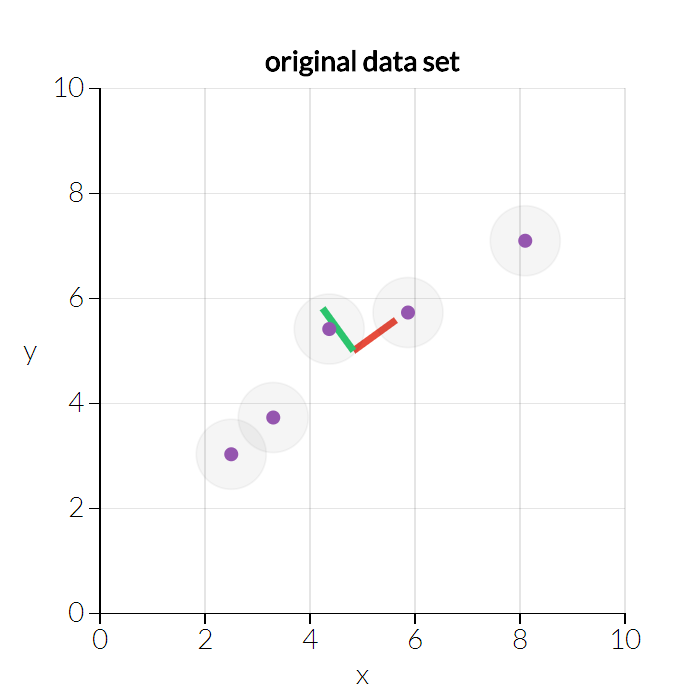
\includegraphics[height=8cm,keepaspectratio]{pcabefore}
% \end{frame}

% \begin{frame}{Principal Component Analysis} 
% 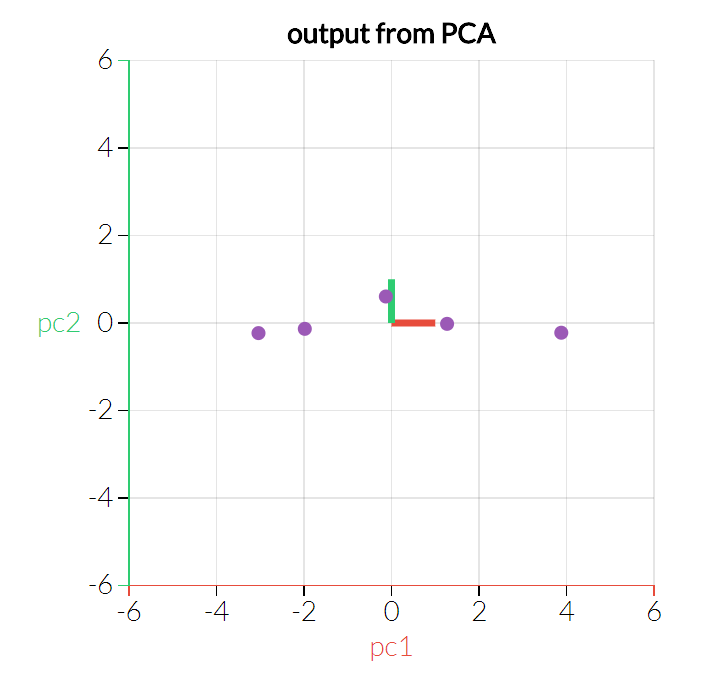
\includegraphics[height=8cm,keepaspectratio]{pcaafter}
% \end{frame}

% \begin{frame}{Principal Component Analysis} 

% \end{frame}

% \begin{frame}{Collaborative Prediction} 

% \end{frame}


% \begin{frame}{Image Compression Using SVD} 
% % https://docs.google.com/viewer?a=v&pid=sites&srcid=ZGVmYXVsdGRvbWFpbnxuYXNsdW5kZXJpY3xneDpkMTI4OTI1NTc4YjRlOGE

% \end{frame}





\section{Generalized Vector}


\begin{frame}{Generalized Arithematic Operations} 

이때까지 벡터, 행렬 등의 \textit{선형대수학적} 객제들의 더하기와 상수배의 operation에 대해서 다루었다. 이제 이 연산을 확장해 보자. 즉, 이제부터는 더하기, 곱하기 등은 굳이 사칙연산일 필요가 없다. 예컨대, 함수끼리의 곱셈을 다음과 같이 정의할 수도 있다. 

$\int f \bullet g dx $ 

더하기 역시 정의하기 나름이다. 이제부터 이러한 일반화된 사칙연산을 고려하기 위한 체계를 세워보겠다. 

\end{frame}

% \begin{frame}{Field} 

% Field는 집합 하나와 그 집합의 원소간의 6개의 연산으로 정의된다. 

% \begin{itemize} 
% \item binary 연산 2개 : 더하기/곱하기 
% \item unary 연산 2개 : 덧셈의 역원/곱셈의 역원 
% \item constant 연산 2개 : 덧셈의 항등원(0) / 곱셈의 항등원(1)
% \end{itemize}

% 이 때, binary 연산은 교환법칙과 결합법칙이 성립해야 하며, 연산의 결과는 언제나 집합의 원소여야만 한다. 

% \end{frame}

\begin{frame}{항등원과 역원} 
어떤 집합 S에서의 이항연산 f에 대해서, 

\begin{itemize} 
\item 집합 S의 모든 원소 s에 대해서 f(s,i) = f(i,s) = s 이면 i를 그 연산의 항등원이라고 한다. 
\item 집합 S의 어떤 원소 s에 대해서 f(s, t) = f(t, s) = i 이면 t를 s의 역원이라고 한다. 
\end{itemize}
\end{frame}

\begin{frame}{Generalized Vector Space} 

어떤 집합 F 위에서 정의된 벡터공간 V는 어떤 집합 V와 F의 원소 a,b 와 V의 원소 $\vec{v}, \vec{u}$에 대해서 다음이 성립하는 벡터연산 더하기와 스칼라곱, 그리고 덧셈의 역원으로 정의된다. 이 때, F를 이 벡터공간의 스칼라라고 한다. 

\begin{itemize} 
\item 벡터덧셈의 교환법칙 / 결합법칙 
\item 벡터덧셈의 항등원 / 역원
\item 스칼라의 곱셈에서의 항등원 1에 대해서, $1\vec{v} = \vec{v}$
\item $(ab)\vec{v} = a(b\vec{v})$ 
\item $a(\vec{v} + \vec{u}) = a\vec{v} + a\vec{u} $
\item $(a+b)\vec{v} = a\vec{v} + b\vec{v}$
\end{itemize}

여기서, 스칼라곱과 벡터-스칼라곱이나 스칼라끼리의 합과 벡터-벡터간의 합은 다른 operation이다. 

\end{frame}

% https://math.okstate.edu/people/binegar/3013-S99/3013-l12.pdf
\begin{frame}{Examples of an Abstract Vector Space} 
\begin{itemize} 
\item Polynomials with degree $\leq n$
\item Matrices
\item Linear Transformations
\item Functions from a specific domain (will be revisited after few weeks)
\item Random Variables (will be revisited after few weeks)
\end{itemize}
\end{frame}

\begin{frame}{예시 : $\mathds{R}^2$에서 $\mathds{R}^2$로의 선형변환}

$\mathds{R}^2$에서 $\mathds{R}^2$로의 선형변환은 2 by 2 행렬로 나타내어질 수 있다. 따라서, 행렬의 덧셈과 실수배를 이용하여 선형변환의 벡터공간을 정의할 수 있다. 이제부터 이 공간의 기저와 좌표, 그리고 2차원 좌표계에서 선형변환 벡터들이 어떠한 의미를 가지는지를 알아볼 것이다. 

\end{frame}

\begin{frame}{예시 : $\mathds{R}^2$에서 $\mathds{R}^2$로의 선형변환} 
먼저, 다음의 행렬들을 생각해 보자. 
$ \vec{e}_1 =  
\left[ \begin{matrix}
1 & 0  \\
0 & 0 
\end{matrix} \right],
\vec{e}_2 = 
\left[ \begin{matrix}
0 & 1  \\
0 & 0 
\end{matrix} \right],
\vec{e}_3 = 
\left[ \begin{matrix}
0 & 0  \\
1 & 0 
\end{matrix} \right],
\vec{e}_3 = 
\left[ \begin{matrix}
0 & 0  \\
0 & 1 
\end{matrix} \right]
$

이 행렬들은 명백하게 2 by 2 행렬이므로, $\mathds{R}^2$에서 $\mathds{R}^2$로의 선형변환이다. 이들 벡터는 선형독립일까? 또, 위 4개의 벡터는 기저가 될까? 
\end{frame}

\begin{frame}{Linear Independence of an Abstract Vector Space}
위 4개의 벡터가 선형독립이기 위해서는 $c_ie_i$을 만족하는 $c_i$가 0뿐이여야 한다. 위 경우, 

$c_i\vec{e}_i = \left[ \begin{matrix}
c_1 & c_2  \\
c_3 & c_4 
\end{matrix} \right]$ 이므로 선형독립임을 알 수 있다. 

또한, 임의의 2 by 2 행렬을 $c_i$를 적절히 조정하여 만들 수 있으므로, 기저임을 알 수 있다. 
\end{frame}



\begin{frame}{예시 : $\mathds{R}^2$에서 $\mathds{R}^2$로의 선형변환} 

위와 같이 선형변환의 기저를 찾은 것은 어떤 의미가 있을까? 

이는 이제부터 우리가 $\mathds{R}^2$의 한 점에서 $\mathds{R}^2$의 한 점으로 대응시키는 선형변환을 언제나 4개의 선형변환을 조합하여 하는 것으로 이해할 수 있다는 점이다. 
\end{frame}


% \begin{frame}{Extending an Abstract Vector Space : Inner Product Space} 
% 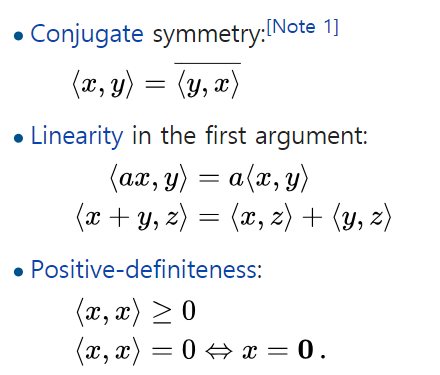
\includegraphics[width=10cm,keepaspectratio]{innerproduct}
% \end{frame}

% \begin{frame}{Abstract Vector Space vs $\mathds{R}^n$}

% \end{frame}


% \begin{frame}{Isomorphism Between Vector Spaces}
% \end{frame}

\begin{frame}{Topics for next lecture} 

\begin{itemize} 
\item Parser Revisited : extending parser
\item 함수의 극한과 미분의 정의. 여러 함수의 미분 및 symbolic 미분기 구현. 
\end{itemize}

\end{frame}

\end{document}


